\documentclass[11pt]{article}

\usepackage{algorithm2e}
\usepackage[english]{babel}
\usepackage{cite}
\usepackage[top=1in,bottom=1in,left=.75in,right=.75in]{geometry}
\usepackage{graphicx}
\usepackage{url}

\bibliographystyle{acm}

\graphicspath{ {figures} }

\begin{document}
\nocite{*}
\begin{titlepage}
\title{Anonymity Analysis of Cryptocurrencies: Master's Thesis Proposal}
\author{Liam Morris \\
  \multicolumn{1}{p{.7\textwidth}}{\centering
  {\tt lcm1115@rit.edu} \\
  \emph{Department of Computer Science, \\
  Rochester Institute of Technology, Rochester, New York}\\\vspace{4em}
  Chair: Professor Stanis{\l}aw Radziszowski\hfill{\tt spr@cs.rit.edu}\\\vspace{1em}
  \hrulefill\\\vspace{1em}
  Reader: Professor Warren Carithers\hfill{\tt wrc@cs.rit.edu}\\\vspace{1em}
  \hrulefill}}
\date{March 3, 2013}
\end{titlepage}
\maketitle
\vspace{6em}
\begin{abstract}
A cryptocurrency is a form of electronic cash backed by mathematical and
cryptographical constructs, unlike traditional currency which was historically
backed by gold or silver. Cryptocurrencies have seen rising popularity in recent
years due to their decentralized, distributed, peer-to-peer protocols. Part of
this rising popularity is also attributable to the supposed anonymity of these
protocols. However, due to the public transaction history required for these
protocols, and the fact that transactions are psuedonymous and not purely
anonymous, this supposed anonymity may not exist. In this thesis we aim to
analyze the technical implementations of Bitcoin and other cryptocurrencies to
determine the level of anonymity provided by these protocols. We also aim to
research some improvements that have already been proposed to determine the
feasibility of such proposals.
\end{abstract}
\thispagestyle{empty}
\clearpage
\pagenumbering{arabic}
\tableofcontents
\listoffigures
\pagebreak
\section{Problem Statement}
A cryptocurrency is a digital currency backed by mathematics and
cryptography, compared to traditional fiat money which was traditionally backed by gold
or silver. The foundation of many cryptocurrencies is based on a key derivation
scheme known as scrypt~\cite{Percival}.
Cryptocurrencies, such as Bitcoin~\cite{Nakamoto08}, provide a means of having a
decentralized, distributed, peer-to-peer electronic cash system. These protocols
supposedly provide some level of anonymity, such that transactions and tender
cannot be directly associated with specific individuals. However, given the
technical specification of many cryptocurrencies, this anonymity may not exist
as stated.

\section{Cryptocurrency Protocols}
Cryptocurrency protocols generally consist of three main components: a
transaction scheme, a verification scheme, and a block chain. The specific
details for each of these may vary between protocols, but they typically exhibit
the same characteristics regardless of specific implementation.

\subsection{Bitcoin Protocol}
Bitcoin is the most widely used cryptocurrency and is the first cryptocurrency
to begin circulation. Many other cryptocurrencies are direct forks of Bitcoin,
so the Bitcoin protocol will be our primary focus.

\subsubsection{Transaction Scheme}
The transaction scheme of Bitcoin uses psuedonyms to specify a transaction
between users on the network. A transaction is recorded as a transfer of some
value from one or more signatures to another signature. 
The method of recording a new transaction of some bitcoin from User A to User
B is as follows:
\begin{enumerate}
    \item User A signs the bitcoin's previous transaction signature with User
        A's private key
    \item The resulting value is used as an input in a hash function along
        with User B's public key
    \item The output of this hash is the transaction signature
\end{enumerate}
\begin{figure}[h]
    \caption{Bitcoin transaction process~\cite{Nakamoto08}}
    \centering
        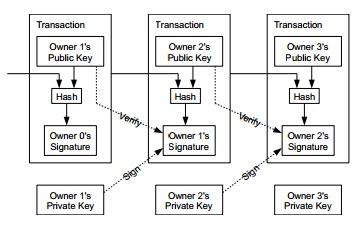
\includegraphics{figures/transaction.png}
\end{figure}

Once a transaction has been created, it is sent out to the Bitcoin network in
order to be verified.

\subsubsection{Verification Scheme}
Once a transaction has been initiated, it must be verified by users in the
Bitcoin network in order for the transaction to be fully committed. Verification
of a transaction requires some proof-of-work in order to complete the block and
append it to the block chain. The proof-of-work scheme used by the Bitcoin
protocol is based on the Hashcash proof-of-work scheme~\cite{hashcash}. 
To complete proof-of-work for some transaction, a
SHA-256 hash with inputs of the previous hash and some nonce must be found such
that the resulting hash is below some difficulty level. In other words, we must
feed the SHA-256 algorithm the previous hash of the coin concatenated with some
nonce such that we have a specified number of leading 0's in the resulting hash.

One common way of computing proof-of-work is using the following algorithm:
\begin{algorithm}
    \KwIn{$D$ = difficulty parameter, $P$ = previous transaction hash}
    \KwOut{nonce, resulting hash}
    $N \gets 0$\\
    $H \gets ${\sc SHA-256($P + N$)}\\
    \While{H $\ge$ D}{
        $N \gets N + 1$\\
        $H \gets ${\sc SHA-256($P + N$)}
    }
    \Return{N, H}
\end{algorithm}

Once a proof-of-work has been determined, the block with the proof-of-work
information is distributed to the Bitcoin network. The difficulty of the
proof-of-work operation is such that blocks are found for a transaction, on
average, in 10 minutes.

\subsubsection{Network Structure}
The original Bitcoin whitepaper~\cite{Nakamoto08} describes the Bitcoin network in the following
way:
\begin{enumerate}
    \item Transactions are broadcast to all network nodes.
    \item Transactions are collected and joined to form a block.
    \item A proof-of-work for a block is found which is broadcast to all nodes.
    \item If the proof-of-work is valid, all transactions in a block are valid,
        and transactions have not already been spent, then block is accepted.
    \item The accepted block is appended to the block chain, and its hash is now
        used as the input hash for the next block.
\end{enumerate}

In other words, all nodes in the network are made aware of new transactions,
verified transactions, and accepted blocks. In this way, the transaction record
(block chain) is shared among all nodes in the network.

\subsection{Litecoin Protocol}
Litecoin is one of the most widely used cryptocurrencies, and is itself a fork
of Bitcoin. The primary difference between Litecoin and Bitcoin is how the coins
are mined, or rather how the transactions are verified. Litecoin aims to have
transactions confirm faster, as well as reduce the benefit of special purpose
hardware for mining coins~\cite{survey}.

\subsubsection{Transaction Scheme}
The Litecoin network method of transaction history is identical to that of
Bitcoin. Litecoin also records the signatures of all users involved, the amount
being transferred, etc.\ in a block, which is then itself part of a larger block
chain.

\subsubsection{Verification Scheme}
Litecoin was forked from Bitcoin to address the strength that special purpose
hardware brings to Bitcoin. Users in the Bitcoin network with application
specific integrated circuits (ASIC) design specifically for computing SHA-256
hashes have an enormous advantage over users without such hardware. To address
this, Litecoin uses the scrypt hashing scheme instead of SHA-256, which changes
the hashing scheme from a CPU-bound operation to a memory-bound operation. By
changing the verification problem from a CPU-hard to memory-hard problem,
parallelization no longer improves the speed of solving the
problem~\cite{Percival}. This yields the following Litecoin proof-of-work
algorithm:
\begin{algorithm}
    \KwIn{$D$ = difficulty parameter, $P$ = previous transaction hash}
    \KwOut{nonce, resulting hash}
    $N \gets 0$\\
    $H \gets ${\sc scrypt($P + N$)}\\
    \While{H $\ge$ D}{
        $N \gets N + 1$\\
        $H \gets ${\sc scrypt($P + N$)}
    }
    \Return{N, H}
\end{algorithm}

\subsubsection{Network Structure}

\subsubsection{Anonymity}
Each transaction contains identifying information with regards to the addresses
of the users. For every transaction in the block chain, we can see between which
users the transaction occurred, as well as the number of bitcoins transferred.
In fact, we can make use of a utility such as~\url{http://blockchain.info} to
search by address to see all transactions that a specific user has made.

\section{Proposed Work}

\bibliography{references}

\end{document}
